\section{A Running Example: Animals}\label{sec:ep}
\begin{figure*}
\centering
\saveSpaceFig
\begin{tabular}{c|c}
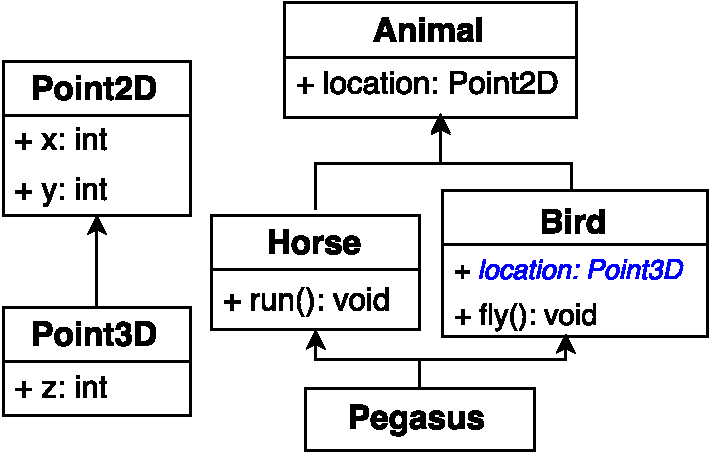
\includegraphics[height=3.3cm]{pdfs/PegasusDetail.pdf}\hspace{0pt} &
\begin{minipage}{7cm}
\vspace{-95pt}
\lstinputlisting[linerange=6-13]{../UseMixinLombok/src/pegasus/simple/java8/Main.java}% APPLY:linerange=PEGASUS_JAVA
%basicstyle=\ttfamily\scriptsize
\end{minipage}
\end{tabular}
\caption{The animal system (left: complete structure, right: code for simplified animal system).}\label{fig:pegasus}
\saveSpaceFig
\end{figure*}

This section illustrates how our programming style, supported by
\mixinAnn{}, enables powerful programming idioms based on multiple
inheritance and type refinements.  We propose a standard example:
\Q@Animal@s with a 2-dimensional \Q@Point2D@ representing their
\Q@location@, subtypes \Q@Horses@, \Q@Bird@s, and \Q@Pegasus@.
Birds can \Q@fly@, thus their locations need to be 3-dimensional
\Q@Point3D@s (field type refinement). We model \Q@Pegasus@
(a well-known creature in Greek mythology) as a kind of
\Q@Animal@ with the skills of both \Q@Horse@s and \Q@Bird@s (multiple
inheritance). A simple class diagram illustrating the basic system is
given on the left side of Figure~\ref{fig:pegasus}.
%\footnote{Some
%  research argues in favor of using subtyping for modeling taxonomies,
%  other research argues against this practice, we do not wish to take
%  sides in this argument, but to provide an engaging example.}

%\bruno{Should we provide a one sentence summary in the abstract of how much code
%is needed in Java (without Obj) vs the approach with CJ, for the Pegasus example?}
%\marco{Not in the abstract. But I think is good to have that number and to put in in the example section.
%I will set up the sentence and someone can compute the number.}

\subsection{Simple Multiple Inheritance with Default
  Methods}\label{sec:simple}

Before modelling the complete animal system, we  start with a
simple version without locations. This version serves the purpose of illustrating how
Java 8 default methods can already model simple forms of multiple inheritance.
\texttt{Horse} and \texttt{Bird} are subtypes
of \texttt{Animal}, with methods \texttt{run()} and \texttt{fly()},
respectively. Pegasus can not only \emph{run} but also \emph{fly}! This is the
place where \emph{``multiple inheritance''} is needed because
\texttt{Pegasus} needs to obtain \texttt{fly} and \texttt{run}
functionality from both \texttt{Horse} and \texttt{Bird}.
A first attempt to model the animal system is given on the right side
of Figure~\ref{fig:pegasus}.
Note that the implementations of the methods \texttt{run}
and \texttt{fly} are defined inside interfaces, using default
methods. Moreover, because interfaces support multiple interface
inheritance, the interface for \texttt{Pegasus} can inherit behaviour
from both \texttt{Horse} and \texttt{Bird}. Although Java interfaces
do not allow instance fields, no form of state is needed so far to
model the animal system.

\para{Instantiation}
To use \texttt{Horse}, \texttt{Bird} and \texttt{Pegasus}, some
objects must be created first. A first problem with using
interfaces to model the animal system is simply that interfaces
cannot be directly instantiated. Classes, such as:

\lstinputlisting[linerange=17-19]{../UseMixinLombok/src/pegasus/simple/java8/Main.java}% APPLY:linerange=PEGASUS_INST

\noindent are needed for instantiation. Now a \texttt{Pegasus} animal can be created
using the class constructor:

\begin{lstlisting}
Pegasus p = new PegasusImpl();
\end{lstlisting}

\noindent There are some annoyances here. Firstly, the sole
purpose of the classes is to provide a way to instantiate
objects. Although (in this case) it takes only one line of code to
provide each of those classes, this code is essentially boilerplate
code, which does not add behavior to the system. Secondly,
the namespace gets filled with three additional types. For example,
both \texttt{Horse} and \texttt{HorseImpl} are needed: \texttt{Horse}
is needed because it needs to be an interface so that \texttt{Pegasus}
can use multiple inheritance; and \texttt{HorseImpl} is needed to
provide object instantiation.
Note that, for this very simple animal system, plain Java 8 anonymous
classes can be used to avoid these problems.  We could have simply
instantiated \texttt{Pegasus} using:

\begin{lstlisting}
Pegasus p = new Pegasus() {}; // anonymous class
\end{lstlisting}

\noindent However, as we shall see, once the system gets a little more
complicated, the code for instantiation quickly becomes more
complex and verbose (even with anonymous classes).

\subsection{Object Interfaces and Instantiation}

To model the animal system with object interfaces all that a user
needs to do is to add an \mixinAnn{} annotation to the \texttt{Horse},
\texttt{Bird}, and \texttt{Pegasus} interfaces:

\lstinputlisting[linerange=8-12]{../UseMixinLombok/src/pegasus/simple/lombok/Main.java}% APPLY:linerange=PEGASUS_LOMBOK
\noindent The effect of the annotations is that a static \emph{factory} method called
\texttt{of} is automatically added to the interfaces. With the
\texttt{of} method a \texttt{Pegasus} object is instantiated as follows:

\begin{lstlisting}
Pegasus p = Pegasus.of();
\end{lstlisting}

\noindent The \texttt{of} method provides an alternative to a
constructor, which is missing from interfaces. The following code
shows the code corresponding to the \texttt{Pegasus} interface
after the \mixinAnn{} annotation is processed:

\begin{lstlisting}
interface Pegasus extends Horse, Bird {
  // generated code not visible to users
  static Pegasus of() { return new Pegasus() {}; }
}
\end{lstlisting}

\noindent Note that the generated code is transparent to users, who
only see the original code with the \mixin annotation. Compared to the pure
Java solution in Section~\ref{sec:simple}, the solution using object interfaces
has the advantage of providing a direct mechanism for object
instantiation, which avoids adding boilerplate classes to the
namespace.

\subsection{Object Interfaces with State}

The animal system modelled so far is a simplified version of the
system presented in the left-side of Figure~\ref{fig:pegasus}.
The example is still not sufficient to appreciate the advantages of IB
programming.
Now we model the complete animal system where an \Q@Animal@ includes a \Q@location@
representing its position in space. We use 2D points to keep track of locations.

\para{\Q@Point2D@: simple immutable data with fields}
Points can be modelled with interfaces.
 In IB
 state is accessed and
manipulated using abstract methods.  The usual approach to model
points in Java is to use a class with fields for the coordinates.
In Classless Java interfaces are used instead:

\begin{lstlisting}
interface Point2D { int x(); int y(); }
\end{lstlisting}

\noindent The encoding over Java is now inconvenient: creating a new point object is cumbersome, even
with anonymous classes:

\begin{lstlisting}
Point2D p = new Point2D() {
  public int x() {return 4;}
  public int y() {return 2;}
}
\end{lstlisting}

\noindent However this cumbersome syntax is not required for every
object allocation. As programmers do, for ease or reuse, the boring
repetitive code can be encapsulated in a method. A generalization of the
\texttt{of} static factory method is appropriate:% in this case:
\begin{lstlisting}
interface Point2D { int x(); int y();
  static Point2D of(int x, int y) {
    return new Point2D() {
      public int x(){return x;}
      public int y(){return y;}
    };  }  }
\end{lstlisting}

\vspace{-5pt}
\para{\Q@Point2D@ with object interfaces}
This obvious ``constructor'' code is generated by the \mixin
annotation.  By annotating the interface \Q@Point2D@, a variation of the shown
static method \texttt{of} will be generated, mimicking the functionality of a
simple-minded constructor. \mixin first looks at the abstract methods and detects
what the fields are, then generates an \Q@of@ method with one parameter for each
of them. We can just write:

\begin{lstlisting}
@Obj interface Point2D { int x(); int y(); }
\end{lstlisting}

\noindent A field or factory parameter is generated for every
abstract method that takes no parameters.
%(except for methods with special
%names).
 An example of using \Q@Point2D@, where we ``clone'' an existing point
 but use
 \Q@42@ as the x-coordinate, is:
\begin{lstlisting}
Point2D p = Point2D.of(42,myPoint.y());
\end{lstlisting}

\para{\texttt{with-} methods in object interfaces}
The pattern of creating a new object by reusing most information from an old
object is very common when programming with immutable
data-structures. As such, it is
supported by \mixin as \Q@with-@ methods:
\begin{lstlisting}
@Obj interface Point2D {
    int x();    int y(); // getters
    // with- methods
    Point2D withX(int val);
    Point2D withY(int val);
}
\end{lstlisting}

\noindent Using \texttt{with-} methods, the point \texttt{p} can also be created
by:

\begin{lstlisting}
Point2D p = myPoint.withX(42);
\end{lstlisting}

\noindent If there is a large number of fields, \texttt{with-} methods
will save programmers from writing large amounts of tedious code that
simply copies field values.
\begin{comment}
is expanded by \mixin into\footnote{
Note how we actually generate a real field \Q@int x=_x;@.
This provides a more uniform translation that can work also for mutable data structures, where setters are required.
}

\begin{lstlisting}
interface Point2D { int x(); int y();
    static Point2D of(int _x, int _y){ return new Point2D(){
        int x=_x; int y=_y;
        public int x(){return x;}   public int y(){ return y; }
        Point2D withX(int val){ return Point2D.of(val,this.y()); }
        Point2D withY(int val){ return Point2D.of(this.x(),val); }
    }; }
  Point2D withX(int val);    Point2D withY(int val); }
\end{lstlisting}
\end{comment}
Moreover, if the programmer wants a different implementation, he may
provide an alternative implementation using \Q@default@ methods. For example:
\begin{lstlisting}
@Obj interface Point2D {
    int x(); int y();
    default Point2D withX(int val){ /*myCode*/ }
    Point2D withY(int val); }
\end{lstlisting}

%\begin{comment}
%\marco{I re-enabled this code, I think is needed for understandability}
\noindent is expanded into
\begin{lstlisting}
interface Point2D {
    int x(); int y();
    default Point2D withX(int val){ /*myCode*/ }
    Point2D withY(int val);
    static Point2D of(int _x, int _y){
      return new Point2D(){
        int x=_x;    int y=_y;
        public int x(){return x;}
        public int y(){return y;}
        public Point2D withY(int val){
          return of(x(),val);}  }; } }
\end{lstlisting}

\noindent Only code for methods needing implementation is generated. Thus,
programmers can easily customize the behaviour for their special needs.
Also, since \mixin interfaces offer the \Q@of@ factory method, only interfaces where all the abstract methods
can be synthesized can be object interfaces. A non-\mixin interface is like an abstract class in Java.
%\end{comment}

%Firstly, to model \texttt{Point2D} that has x-coordinate and y-coordinate by an
%interface, we immediately run into the problem of expressing the fields
%\texttt{x} and \texttt{y}.
%interfaces. Method \texttt{withX, withY} creates a new instance of
%\texttt{Point2D} with updated field \texttt{x,y}, respectively.

% Firstly, to model \texttt{Animal} by an interface, we immediately run into the
% problem of expressing the field \texttt{point}. Since in Java there is no way to
% define member fields inside interfaces, we propose to simulate fields by
% abstract methods inside interfaces:

%\lstinputlisting[linerange=42-48]{../UseMixinLombok/src/pegasus/TestAnimal.java}% APPLY:linerange=POINT2D

%\paragraph{Instantiation}
%In Java, to implement an interface like \texttt{Point2D}, a typical and trivial
%approach that programmers usually do is creating a class extending the interface
%and providing implementation for all methods inside. For example, this is the
%implementation for interface \texttt{Point2D}:

%\begin{lstlisting}
%class Point2DImpl implements Point2D {
%    private int _x;
%    private int _y;
%    public Point2DImpl(int x, int y) {
%        this._x = x;
%        this._y = y;
%    }
%    public int x() {
%        return _x;
%    }
%    public int y() {
%        return _y;
%    }
% %Your implementation of with is wrong
%    public Point2D withX(int x) {
%        x(x);
%        return this;
%    }
%    public void x(int x) {
%        _x = x;
%    }
%    public void y(int y) {
%        _y = y;
%    }
%    public Point2D withY(int y) {
%        y(y);
%        return this;
%    }
%}
%\end{lstlisting}
%
%\texttt{Point2DImpl} implements \texttt{Point2D} and provides a constructor with
%quite mechanical code. What's worse, the implementation in \texttt{Point2DImpl}
%may not be reused in a single inheritance language.

%
%\begin{lstlisting}
%  // inside interface Point2D
%  static Point of(int x, int y) {
%      return new Point() {
%          int _x = x;
%          int _y = y;
%          public int x() {
%            return _x;
%          }
%          public int y() {
%            return _y;
%          }
%          public Point2D withX(int x) {
%            x(x);
%            return this;
%          }
%          public void x(int x) {
%            _x = x;
%          }
%          public void y(int y) {
%            _y = y;
%          }
%          public Point2D withY(int y) {
%            y(y);
%            return this;
%          }
%    }
%  }
%\end{lstlisting}
%
%\lstinputlisting[linerange=-]{} % APPLY:linerange=POINT_OF

\para{\Q@Animal@ and \Q@Horse@: simple mutable data with fields}
2D points are mathematical entities, thus we choose an immutable data structure to
model them. Animals are real world entities, and when an animal moves,
it is the \emph{same} animal with a different location. We model this with
mutable state.

%Now we proceed to define \texttt{Animal} with \texttt{point} ``member
%field''.
%%Not again, before we used only getters!
% Again, we model this member field with getter and setter methods:
\lstinputlisting[linerange=58-60]{../UseMixinLombok/src/pegasus/TestAnimal.java}% APPLY:linerange=ANIMAL

\noindent Here we declare an abstract getter and a setter for the mutable ``field''
\Q@location@.  Without the \mixin annotation, there is no convenient way to
instantiate \texttt{Animal}.  For \texttt{Horse}, the \mixin annotation is used
and an implementation of \texttt{run()} is defined using a \Q@default@
method. The implementation of \texttt{run()} further illustrates the convenience of \texttt{with-} methods:

\lstinputlisting[linerange=64-66]{../UseMixinLombok/src/pegasus/TestAnimal.java}% APPLY:linerange=HORSE

\noindent Creating and using \texttt{Horse} is quite simple:

\lstinputlisting[linerange=10-12]{../UseMixinLombok/src/pegasus/TestAnimal.java}% APPLY:linerange=USINGHORSE

\noindent Note how the \texttt{of}, \texttt{withX} and
\texttt{location} methods (generated automatically) give a
basic interface for dealing with animals.

In summary, state (mutable or not) in object interfaces
relies on a notion of abstract state, and state is not directly
available to programmers. Instead programmers use methods, called
\emph{abstract state operations}, to interact with state.

% by method
%\texttt{run()}: method \texttt{withX} returns a new point object with field
%\texttt{x} updated by the argument to \texttt{withX}. Without these
%\texttt{with} methods, operations like \texttt{run()} would be much harder to define.

\subsection{Object Interfaces and Subtyping}
\Q@Bird@s are \Q@Animal@s, but while \Q@Animal@s only need 2D
locations, \Q@Bird@s need 3D locations. Therefore when the \texttt{Bird}
interface extends the \Q@Animal@ interface, the notion of points needs to
be \emph{refined}. Such kind of refinement is challenging
in typical \classbased approaches. Fortunately, with object interfaces,
we are able to provide a simple and effective solution.

\para{Unsatisfactory \classbased solutions to field type refinement}
In Java if we want to define an animal class with a field we have a set of
unsatisfactory options in front of us:
\begin{itemize}
\item Define a \Q@Point3D@ field in \Q@Animal@: this is bad since all animals
  would require more than needed.
  %Also it requires the programmer to predict the future, or
  Also it requires adapting the old code to accommodate for new evolutions.

\item Define a \Q@Point2D@ field in \Q@Animal@ and define an extra \Q@int z@
  field in \Q@Bird@.  This solution is very ad-hoc, requiring to basically
  duplicate the difference between \Q@Point2D@ and \Q@Point3D@ inside \Q@Bird@.
  %Again, there are many reasons this would be bad,
  The most dramatic criticism is that it would not scale to a scenario when
  \Q@Bird@ and \Q@Point3D@ are from different programmers.

\item Redefine getters and setters in \Q@Bird@, always put \Q@Point3D@ objects
  in the field and cast the value out of the \Q@Point2D@ field to \Q@Point3D@
  when implementing the overridden getter.  This solution scales to the multiple
  programmers approach, but requires ugly casts and can be implemented in a
  wrong way leading to bugs.
\end{itemize}

We may be tempted to assume that a language extension is needed.
%Instead, with object interfaces, another approach is possible
Instead, the \emph{restriction} of (object) interfaces to have no
fields enlightens us that another approach is possible; often in programming languages ``freedom is slavery''.

\para{Field type refinement with object interfaces}
Object interfaces address the challenge of type-refinement as follows:
\begin{itemize}
\item by \emph{covariant method overriding}, the return type of
  \texttt{location()} is refined to \texttt{Point3D};
\item by \emph{overloading}, a new setter for location is defined with a more
  precise type;
\item a \Q@default@ setter implementation with the old signature is provided.
\end{itemize}

\noindent Thus the code for the \Q@Bird@ interface is:

\lstinputlisting[linerange=70-79]{../UseMixinLombok/src/pegasus/TestAnimal.java}% APPLY:linerange=BIRD
%Interface \texttt{Point3D} extends \texttt{Point2D} with a new abstract method
%\texttt{int z()} (treated as a getter for member field \texttt{z}). Note that
%the return type of various methods (e.g. with- methods, getters) get refined
%either by covariant method overriding or automatically by our annotation
%processor. Besides \emph{with}, other methods (including \emph{clone},
%\emph{of}) also do type-refinements automatically.


\noindent From the type perspective, the key is the covariant method
overriding of \texttt{location()}. However, from the semantics
perspective the key is the implementation for the setter with the old
signature (\Q@location(Point2D)@). The key to the setter
implementation is a new type of \Q@with@ method, called
 a (functional) property updater.

\para{\Q@Point3D@ and property updaters}
The \Q@Point3D@ interface is defined as follows:

\lstinputlisting[linerange=52-55]{../UseMixinLombok/src/pegasus/TestAnimal.java}% APPLY:linerange=POINT3D

\noindent \Q@Point3D@ includes a
\Q@with@ method, taking a \Q@Point2D@ as an argument.
Other wither methods (such as \Q@withX@) functionally update a field one at a time.  This can be
inefficient, and sometimes hard to maintain.  Often we want to update multiple
fields simultaneously, for example using another object as source.  Following
this idea, the method \Q@with(Point2D)@ is an example of a (functional)
property updater: it takes a certain type of object and returns a copy of the
current object where all the fields that match fields in the parameter
object are updated to the corresponding value in the parameter. The idea is that
the result should be like \Q@this@, but modified to be as similar as possible to the parameter.

With the new \Q@with@ method we may use the information for
\Q@z@ already stored in the object to forge an appropriate \Q@Point3D@
to store. Note how all the information about what fields sit in
\Q@Point3D@ and \Q@Point2D@ is properly encapsulated in the
\Q@with@ method, and is transparent to the implementer of \Q@Bird@.

Property updaters never break class invariants, since they
internally call operations that were already deemed
safe by the programmer. For example a list object
would not offer a setter for its \texttt{size} field (which should be kept hidden), thus
a property updater would not attempt to set it.

% To implement the old setter in a convenient way, \mixin supports one
% last type of operations: property updater \texttt{with}
% methods. Unlike the \texttt{withX} (where \texttt{X} stands for a
% field name) methods presented so far, property updaters take several
% fields at once, contained in an interface, and copy those fields into
% fields of another interface.

%Symmetrically, we could offer an imperative property updater that
%calls the setters instead of the withers.  \Q@Point3D set(Point2D
%val)@.

\begin{figure}
\saveSpaceFig
\lstinputlisting[linerange=88-114]{../UseMixinLombok/src/pegasus/TestAnimal.java}% APPLY:linerange=GENERATED_POINT3D
\caption{Generated boilerplate code.}
\label{fig:boilerplate}
\saveSpaceFig
\end{figure}

\para{Generated boilerplate}
To give an idea of how much code \mixin is generating, we show the
generated code for \texttt{Point3D} in Figure~\ref{fig:boilerplate}.
%\marcoT{Overall, for the whole
%animals-with-locations, an @@@ lines code example,
%the generate/completed code is composed by
%@@@ lines.}
Writing such code by hand is error-prone. For
example a distracted programmer may swap the arguments of calls to
\Q@Point3D.of@.  Note how \Q@with-@ methods are automatically refined in their
return types, so that code like:

\begin{lstlisting}
Point3D p = Point3D.of(1,2,3); p = p.withX(42);
\end{lstlisting}

\noindent will be accepted. If the programmer wishes to suppress this behavior
and keep the signature as it was, it is sufficient to redefine the \Q@with-@
methods in the new interface repeating the old signature.  Again, the philosophy
is that if the programmer provides something directly, \mixin does not touch it.
The cast in \Q@with(Point2D)@ is trivially safe because of the \Q@instanceof@
test. The idea is that if the parameter is a subtype of the current exact type,
then we can just return the parameter, as something that is just ``more'' than
\Q@this@.

\begin{figure*}
\saveSpaceFig
\centering
\hspace{.01in}{%\fontsize{8}{10}\selectfont
\begin{tabular}{|l|l|l|l|}
\hline
& \textbf{Operation}  & \textbf{Example}                  & \textbf{Description } \\ \hline
\multirow{4}{*}{\parbox{2.3cm}{State operations (for a field \texttt{x})}} & \textbf{``fields''/getters}        &   \Q@int x()@                  & Retrieves value from field \texttt{x}.          \\ \cline{2-4}
& {\bf withers}        &   \Q@Point2D withX(int val)@                & Clones
object; updates field \texttt{x} to \texttt{val}.             \\ \cline{2-4}
& \textbf{setters}        & \Q@void x(int val)@ & Sets the field
\texttt{x} to a  new value \texttt{val}.        \\ \cline{2-4}
& \textbf{fluent setters}        & \Q@Point2D x(int val)@ &Sets the field
\texttt{x} to \texttt{val} and returns \texttt{\this}.  \hspace{-.1in}         \\ \hline
\multirow{3}{*}{Other operations} &
\textbf{factory methods} &
%\begin{tabular}{l}
\Q@static Point2D of(int _x,int _y)@
%\end{tabular}
 & Factory method (generated).        \\
\cline{2-4}
& \textbf{functional updaters}        & \Q@Point3D with(Point2D val)@
& Updates all matching fields in \texttt{val}.        \\ \hline
%\cline{2-4}
%& \textbf{imperative updaters}        & \Q@Point3D set(Point2D val)@ &
%Set all matching fields in \texttt{val}.        \\ \hline
\end{tabular}
}
\caption{Abstract state operations for a field \texttt{x}, together with other operations, supported by the \mixin
  annotation. }

\label{fig:abstractstate}

\end{figure*}

\para{Summary of operations in Classless Java}
%Method bodies can only refer to other methods;
%Objects are (conceptually) closures and the state is
%composed by captured local variables.}
%Methods interacting with state are called \emph{abstract state operations}.
In summary, object interfaces provide support for
different types of abstract state operations: four field-based state
operations; and functional updaters. Object instantiation is directly
supported by \texttt{of} factory methods.
Figure~\ref{fig:abstractstate} summarizes the six operations supported
by \mixin. The field-based abstract state operations are determined by
naming conventions and the types of the methods. Fluent setters are a variant of
conventional setters, and are discussed in more detail in Section~\ref{sec:dsls}.

\begin{comment}
\textcolor{red}{Note that we are breaking the naming conventions for getters and setters in Java;
they have the same names as their fields in our case, which makes code more concise,
but also presents a nice form of fluent setters with method chaining (see Section~\ref{sec:dsls}).
Fluent setters are useful, and the difference from \Q@with-@ methods is that they do not create new objects.}
\end{comment}

\subsection{Advanced Multiple Inheritance}
Finally, defining \texttt{Pegasus} is as simple as we did in the simplified
(and stateless) version on the right of Figure~\ref{fig:pegasus}.
 Note how even the non-trivial pattern for field type refinement is
transparently composed, and \texttt{Pegasus} has a \Q@Point3D@
\Q@location@.%  This works because \Q@Horse@ do not perform
% any field type refinement, otherwise we may have to choose/create a
% common subtype in order for \texttt{Pegasus} to exists.

\lstinputlisting[linerange=83-83]{../UseMixinLombok/src/pegasus/TestAnimal.java}% APPLY:linerange=PEGASUS


\begin{comment}
\subsection{A Running Example: \texttt{Point}}
Suppose we want to create a point component that models the a point in space,
that has x-coordinate and y-coordinate. For example, if we create the
\texttt{Point} interface in Java, it would look like this:

\begin{lstlisting}
interface Point {
    int x();
    int y();
}
\end{lstlisting}

\texttt{Point} has two (conceptually) member fields \texttt{x} and \texttt{y},
representing the two coordinates of a point. Methods \texttt{int x()} and
\texttt{int y()} serve as \emph{getter} methods.
% Methods \texttt{void X(int X)} and \texttt{void Y(int Y)} serve as
% \emph{setter} methods. Method \texttt{Point withX(int X)} updates field
% \texttt{X} and returns \textbf{this}.

\subsection{Naive Implementation}
In Java, to implement an interface like \texttt{Point}, a typical and trivial
approach that programmers usually do is creating a class extending the interface
and providing implementation for all methods inside. For example, this is the
implementation for interface \texttt{Point}:

\lstinputlisting[linerange=-]{} % APPLY:linerange=POINTIMPL

\texttt{PointImpl} implements \texttt{Point} and provides a constructor with
quite mechanical code. What's worse, the implementation in \texttt{PointImpl}
may not be reused in a single inheritance language.

\subsection{The Classless Java Approach}
Instead of writing a whole another class to provide the implementation for
\texttt{Point}, we annotate on interface \texttt{Point} directly with \mixin:

\lstinputlisting[linerange=-]{} % APPLY:linerange=POINT

The \mixin annotation will generate a static method \texttt{of} inside
\texttt{Point}. The method \texttt{of} mimic the functionality of constructors,
it takes arguments same as constructors and return objects similar to
constructors. It makes use of Java anonymous classes and achieves the same
implementation as \texttt{PointImpl}.

With \CJ, we provide a Java annotation \mixin to provide default
implementations for various methods and a mechanism to instantiate
objects. \mixin annotation helps programmers to write less cumbersome code and
instantiate interfaces in Java.

\lstinputlisting[linerange=-]{} % APPLY:linerange=POINT_OF
\end{comment}


\begin{comment}
\subsection{More On \mixin}
Besides the benefit of freeing programmers from writing boilerplate code, our
\mixin annotation can also allow programs to mimic multiple inheritance in a
restricted form easily.

\lstinputlisting[linerange=42-48]{../UseMixinLombok/src/pegasus/TestAnimal.java}% APPLY:linerange=POINT2D

\lstinputlisting[linerange=52-55]{../UseMixinLombok/src/pegasus/TestAnimal.java}% APPLY:linerange=POINT3D

\lstinputlisting[linerange=58-60]{../UseMixinLombok/src/pegasus/TestAnimal.java}% APPLY:linerange=ANIMAL

\lstinputlisting[linerange=64-66]{../UseMixinLombok/src/pegasus/TestAnimal.java}% APPLY:linerange=HORSE

\lstinputlisting[linerange=70-79]{../UseMixinLombok/src/pegasus/TestAnimal.java}% APPLY:linerange=BIRD

\lstinputlisting[linerange=83-83]{../UseMixinLombok/src/pegasus/TestAnimal.java}% APPLY:linerange=PEGASUS

Interface \texttt{Point3D} extends \texttt{Point/Point2D} with a new abstract
method \texttt{int z()} (treated as a getter for member field
\texttt{z}). Interface \texttt{Horse} shows the usage and advantage of
\emph{with} methods by method \texttt{run()}: method \texttt{withX} returns a
new point object with field \texttt{x} updated by the argument to
\texttt{withX}. Without these \texttt{with} methods, operations like
\texttt{run()} would be much harder to define. Note that the return type of
various methods get refined automatically by our annotation processor. Besides
\emph{with}, other methods (including \emph{clone}, \emph{of}) also do
type-refinements automatically.

The \emph{``multiple inheritance''} case appears at interface
\texttt{Pegasus}. Pegasuses can not only \emph{run} but also \emph{fly}!
Interface \texttt{Pegasus} obtains \texttt{fly} and \texttt{run} functionality
through interface \texttt{Horse} and \texttt{Bird}. Using \mixin annotation,
actually there is no code that programmers have to write at all. The idea of using
default methods inside interfaces was proposed in ~\cite{}. It enables us to do
multiple inheritance, which otherwise is hard to do in Java-like languages that
do not support multiple inheritance, easily.
\end{comment}

